\chapter{Project Overview}\label{chap:Overview}

The main project description we started to work with was quite short with about 300 words and was also hugely complemented and clarified in meetings with Prof. Weber-Wulff. Nonetheless it contains very important parts that are the foundation of what was built during the project:

\begin{quote}
\enquote{Right. I'm the plagiarism \enquote{huntress}. I've tested plagiarism detection software since 2004. Mostly, they suck. They either don't work, or are a pain to use, or both. I've spent 10 years trying to educate people about plagiarism, and still the media thinks I have a magic secret for discovering plagiarism, as demonstrated on the GuttenPlagWiki and the VroniPlagWiki. What actually happens there is that quite a number of tools are used for preparing texts, discovering possible sources, comparing them, and documenting them. The last part is done by hand and takes an enormous amount of time.

The idea is to set up a Plagiarism Detection Cockpit that integrates all sorts of bits and pieces, but leaves the teacher in command. It is not to be a general test system that spits out a number for every paper submitted, although the integration of as many such systems as possible will be one of the necessary features of the system. There will be a lot of thought needed for the interface design, as there are massive amounts of data that need to be displayed. How can this be compressed and fit on a screen? For example, a barcode-generation needs to be integrated.

The goal will be to provide a tool that easily produces simple-to-read 
documentation and deals with all sorts of nastiness that might 
turn up on the way. The tool must be multi-lingual and open source.
 It would also be cool to integrate some of the little tools such 
 as the Android-based OCR-Scanner that was developed in the SS 2011. 
 I would like for the team to use an agile development methodology 
 so that we can continuiously test with teachers and professors 
 and *Plaggers.

One of the first tasks will be collecting up the computing 
literature on the topic of plagiarism discovery. A wiki needs to 
be set up with links to material (online and offline), comments on 
the papers, and as many navigational indices as possible.}\citep{projectDescription}
\end{quote}\label{cite:projectDescription}

In the beginning the main takeaways we used from this text were:

\begin{itemize}
\item \textbf{no} automated process, \enquote{just} a tool that aids the users workflow
\item needs an open source license
\item multi language support
\end{itemize}

If you read the text carefully though, you may notice that we 
overlooked or at least marginalized some important clues, but you 
will find descriptions of those problems later on in the chapter \nameref{chap:summaryAndOutlook}.

One important information that was only stated during the first project proposal was, that it also needed to be web based.

For the frontend this made the choices of languages and technologies pretty easy, because there are some clear web standards, without much alternatives aside from the version numbers. As we wanted to develop in a future-proof manner and chose to support only from Internet Explorer 8 upwards, this lead us to CSS3 for styling, HTML5 for the markup and JavaScript for client-side scripting. With JavaScript being the only one of those three with a real competitior in \href{http://www.dartlang.org/}{Googles Dart}, but as the browser support is still very weak, 
this wasn't a possibility.

On the server-side however the possibilities for programming languages and platforms are a little bit broader than this. The most
important criterias for us regarding those choices were, that it had to be flexible and already very widespread, because this would be helpful for an open source project to gather a community later on.

From the twenty most used programming languages according to \citet{tiobe} only PHP, Ruby, JavaScript(with \href{http://nodejs.org/}{Node.js}), Java and Python seemed really suitable for web development. Naturally the familiarity and preferences of the team members also played a role in the final decision. We made bad experience with Java in this area and felt that structuring JavaScript and Python in a big application could be problematic. From the two
languages that were left, the one we had the most experience with and that also has the 
biggest following was PHP, so it made the final cut.

For the \enquote{platform} we only made the decision to use Apache as the web server, because it is the most common\citep{webServers} and it also runs on many different operating systems, so that the real platform choice doesn't need to be made.

As you will see below, the usage of a database was also made in a flexible way. We currently use MySQL, but it should be possible to swap the storage engine easily if necessary.

\section{Statistics}

We gathered some data of the state of Unplagged as of July 7th 2012 with the tool \href{http://cloc.sourceforge.net/}{Count Lines of Code(CLOC)}. We know that by no means this can be used as a quality measurement, but we believe that it can give some structural insights and is a good starting point for an introduction of the technical area.


\begin{figure}[!h]
  \centering
\begin{tabular}{lrrr}
\toprule
Language & Files & Comments & Code \\
\midrule
PHP & 3262 & 275579    &     429308 \\
XML & 194 & 0 & 234696 \\
HTML                     &         2645       &     191     &     24684 \\
CSS                      &         1220      &      843     &      7093 \\
Javascript                & 59       &       1932     &      5239 \\
XSD                      &           108     &         6       &    1058 \\
SQL                    &        49        &     58      &      102 \\
C                      &            18           &  16       &      72 \\
make                  &                     4      &       4    &         13 \\
\midrule
Sum: & 4013 & 278629 & 702265 \\
\bottomrule
\end{tabular}
  \caption{Complete measurements including library/framework files}
  \label{tab:completeMeasure}
\end{figure}

The table in figure \ref{tab:completeMeasure} shows the complete(At least according to CLOC) count of files, comment lines and lines of code, that are currently part of Unplagged. It contains also all the code 
that is part of all used libraries or frameworks.

In all the following pie charts the measurements you will see are narrowed down as much as possible\footnote{CLOC was called with the following arguments: perl /cloc-1.56.pl application tests scripts public library/Unplagged --force-lang=html,phtml --exclude-dir=libs} to contain only code that was created by members of the team.

\begin{figure}[!h]
  \centering
    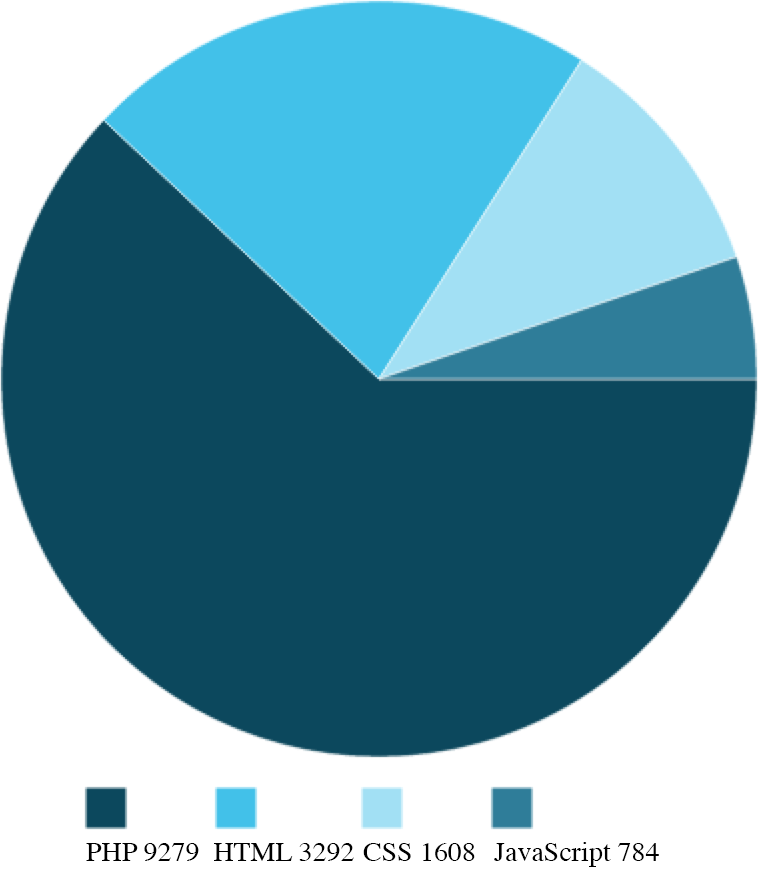
\includegraphics[width=0.55\textwidth]{images/loc.png}
  \caption{Distribution of created lines of code by language.}
  \label{fig:locDistribution}
\end{figure}

As you can see when comparing the numbers in figure \ref{fig:locDistribution} with the table, we are really standing on the shoulders of giants as is often said, with just about 2.1\% of the whole PHP code written by us for example.

\begin{figure}[!h]
  \centering
    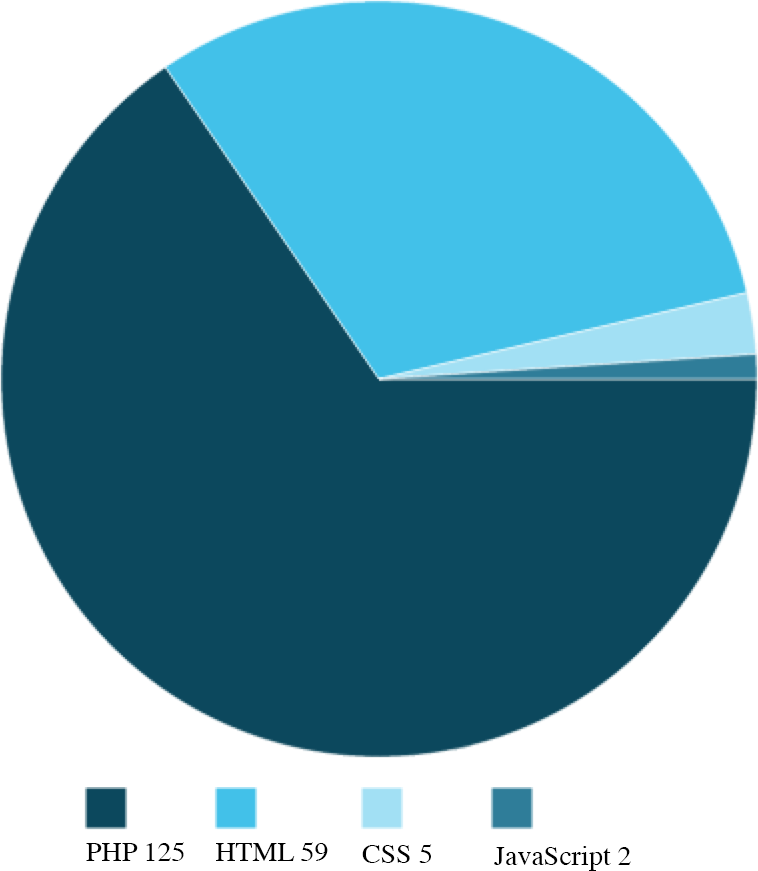
\includegraphics[width=0.55\textwidth]{images/files.png}
  \caption{Distribution of self created files in Unplagged.}
  \label{fig:fileDistribution}
\end{figure}

What could be a bit misleading is the count of HTML files and lines, because they mostly contain some kind of mish-mash of PHP and HTML, including some simple loops to generate recurring elements.

For the main architecture of the system that lies in the PHP part, we feel that the ratio of 125 files(see figure \ref{fig:fileDistribution}) to 9279 lines of code(see figure \ref{fig:locDistribution}) or ca. 75 lines of actual code per file is a pretty good achievement, as it is at least an indicator of a good software design. For JavaScript and CSS the numbers 
are not that great, but this happened mostly due to performance concerns, because it is 
really desirable to reduce HTTP requests the client has to make, which can be easily done by putting it all in very big files.

With comments it's even more complicated to judge the quality by pure numbers of lines,
because they are just there and have no \enquote{understanding ratio} of readers that could be easily measured, but to complete this short excursion into statistical territory: In figure \ref{fig:commentDistribution}, you can see the distribution of comments by language, with PHP again leading the pack by far.

\begin{figure}[!h]
  \centering
    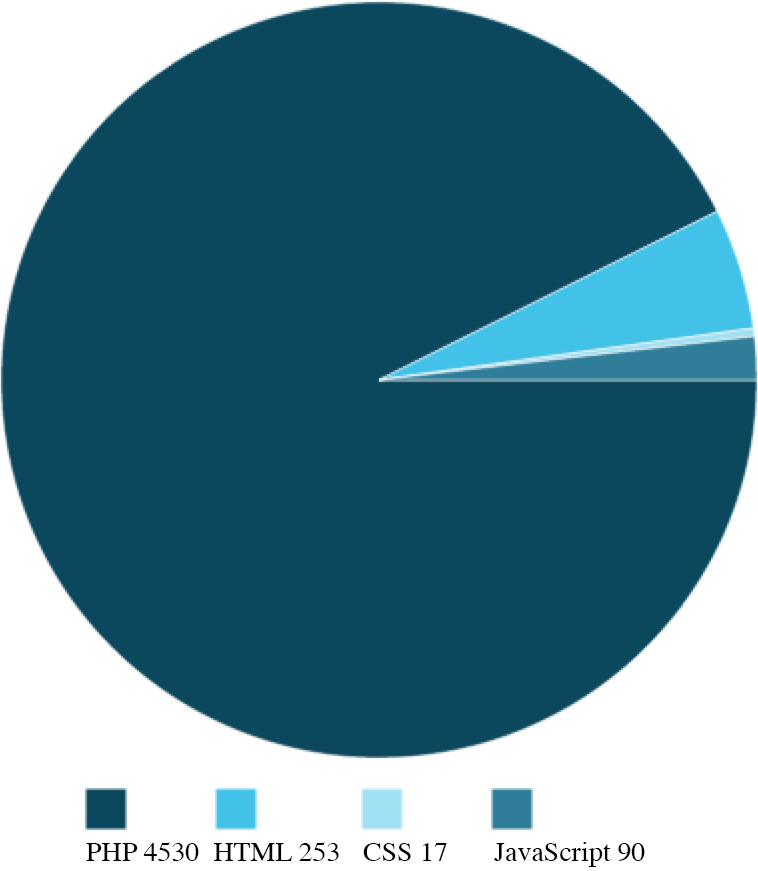
\includegraphics[width=0.55\textwidth]{images/comments.png}
  \caption{Distribution of comment lines by language.}
  \label{fig:commentDistribution}
\end{figure}

\section{Licensing -- GPLv3}

Choosing an open source license was something that was surprisingly difficult for us,
because we never had to do it before and there are so many different possibilites out there with many upsides and downsides.

We eventually decided to use the GNU Public License in version 3(GPLv3). The reasons for this choice are the very widespread usage of it, meaning that many people are already 
familiar with it, the international validity of the specified terms and the \enquote{viral}
character of it, so that any additions and changes to the software also need to be provided 
under the same open source license.

It has therefore the benefit of keeping the possibility to dual-license the system with another proprietary license later on in order to maybe even sell it to organizations that want to include
customizations without making them public, which would be mandatory under the GPLv3, but making it freely available to others that operate under the specified terms.

\section{Project Structure and Technologies}

Over the course of the project we integrated something that could be called \enquote{toolbox} of libraries and frameworks, which 
helped us develop faster, more efficient or according to some kind of \enquote{best-practices}
in some areas.

\begin{figure}[!h]
\dirtree{% 
.1 unplagged/.
.2 application/.
.3 configs/.
.3 controllers/.
.3 forms/.
.3 layouts/.
.3 models/.
.3 views/.
.2 data/.
.2 docs/.
.2 library/.
.2 public/.
.3 images/.
.3 js/.
.3 style/.
.3 index.php.
.2 scripts/.
.2 tests/.
.2 gpl-3.0.txt.
.2 readme.txt.
}
\caption{Most important directores of Unplagged}
  \label{fig:directoryStructure}
\end{figure}

The main directory structure you can see in figure \ref{fig:directoryStructure} is mostly like the one recommended by the Zend framework documentation\footnote{http://framework.zend.com/manual/en/project-structure.project.html}, which is a major building block of 
Unplagged and the first thing we integrated.

Most of the custom code that we wrote lies in the \texttt{application} directory and \texttt{library} contains nearly all the foreign code.

Public resources like CSS, JavaScript and some image files are all served from the \texttt{public/} directory, so the web server must be configured correctly to use this directory as the webroot. Every request that is made to the application is routed through the \texttt{index.php} file in this directory as well and then dispatched to Zend framework.

\subsection{Zend Framework}

Zend is a collection of PHP classes, that can be used in two different ways, first as a simple set of libraries, of which we for example made use for translating the application into different languages, creating webforms or for the rights management. But second, and more importantly, it also provides a framework for a MVC application, which automatically routes URLs according to a scheme into the correct controller classes.

It has some competitors mainly in \href{http://cakephp.de/}{CakePHP}, but they essentially have the same features, so this choice was again more a matter of taste and experience.

\subsection{Doctrine ORM}

This can as well be used in different ways, but for our purposes, the most important bit was the possibility to write plain old PHP classes and annotate them in a way that maps them to database tables. Through this mechanism it is possible to generate the whole database by calling one simple script with the credentials of the database and have therefore flexibility regarding the used DBMS.

\subsection{HTML5 Boilerplate}

The HTML5 Boilerplate was the starting point for our front end development and is a pretty nice collection of best-practices mostly for CSS and HTML. It contains for example a CSS reset that tries to bring the default styles of all HTML elements for every browser to the same point, some basic CSS classes for image replacements or clearing floats and ways to target older browsers via specific CSS classes.

\subsection{jQuery}

Essentially all the JavaScript we wrote could be written without jQuery. The main benefit it brings though, is that it hides the differences between the JavaScript implementations of different browsers, so that coding gets much more comfortable and robust.

Besides this, jQuery also provides a nice set of animations, that in some cases and if not used excessively, can help make the user interface a little nicer.

\subsection{Twitter Bootstrap}

Twitter Bootstrap is a set of mostly CSS components that was integrated very late, about six or seven month into the project, and replaced the buttons and error messages we already had built. This was primarily done because the usability of those elements had a much nicer flow and the browser compatibility was also more robust out of the box.
Later on we also used it also on some more components like dialogs and the paging element.

The problem with Bootstrap is, that webpages that use it tend to look very uniform, because of all the similar looking elements, but we made this choice here, because we felt that for a webapp the usability is more important than a unique design. And hopefully we also kept some uniqueness to it.

\subsection{Responsive Design}

Responsive Design isn't really a tool or framework like all the others described here, but more a paradigm regarding the way a webpage is styled via CSS. It means that CSS media queries are used to target specific viewport widths, so that no matter what device is used to view the application, the page always has an optimized layout.